
//Intro results


\subsection{SHM relation}
The SHM relation from TNG is plotted in Figure \ref{shmr_res}, along with the best fits from \textcite{Behroozi2013} and \textcite{Zanisi2019}.
When calculating the SHM relation using all the galaxies, the median values are pushed towards lower halo masses compared to only central galaxies. For $M_{halo} > 10^{12} M_{\odot}$, the TNG SHM relation deviates significantly from the abundance matching fit by having a much steeper slope. This indicates a value for $\gamma$ in equation \ref{eq_behroozi} closer to unity. The more recent results from \textcite{Zanisi2019} agrees better with the high mass slope than the other two, but the difference is still significant. The result is expected, as TNG has been found to produce galaxies with too high stellar mass in larger subhalos. This might indicate a too high star formation rate in these galaxies.


\begin{figure}
    \centering
    \makebox[\textwidth][c]{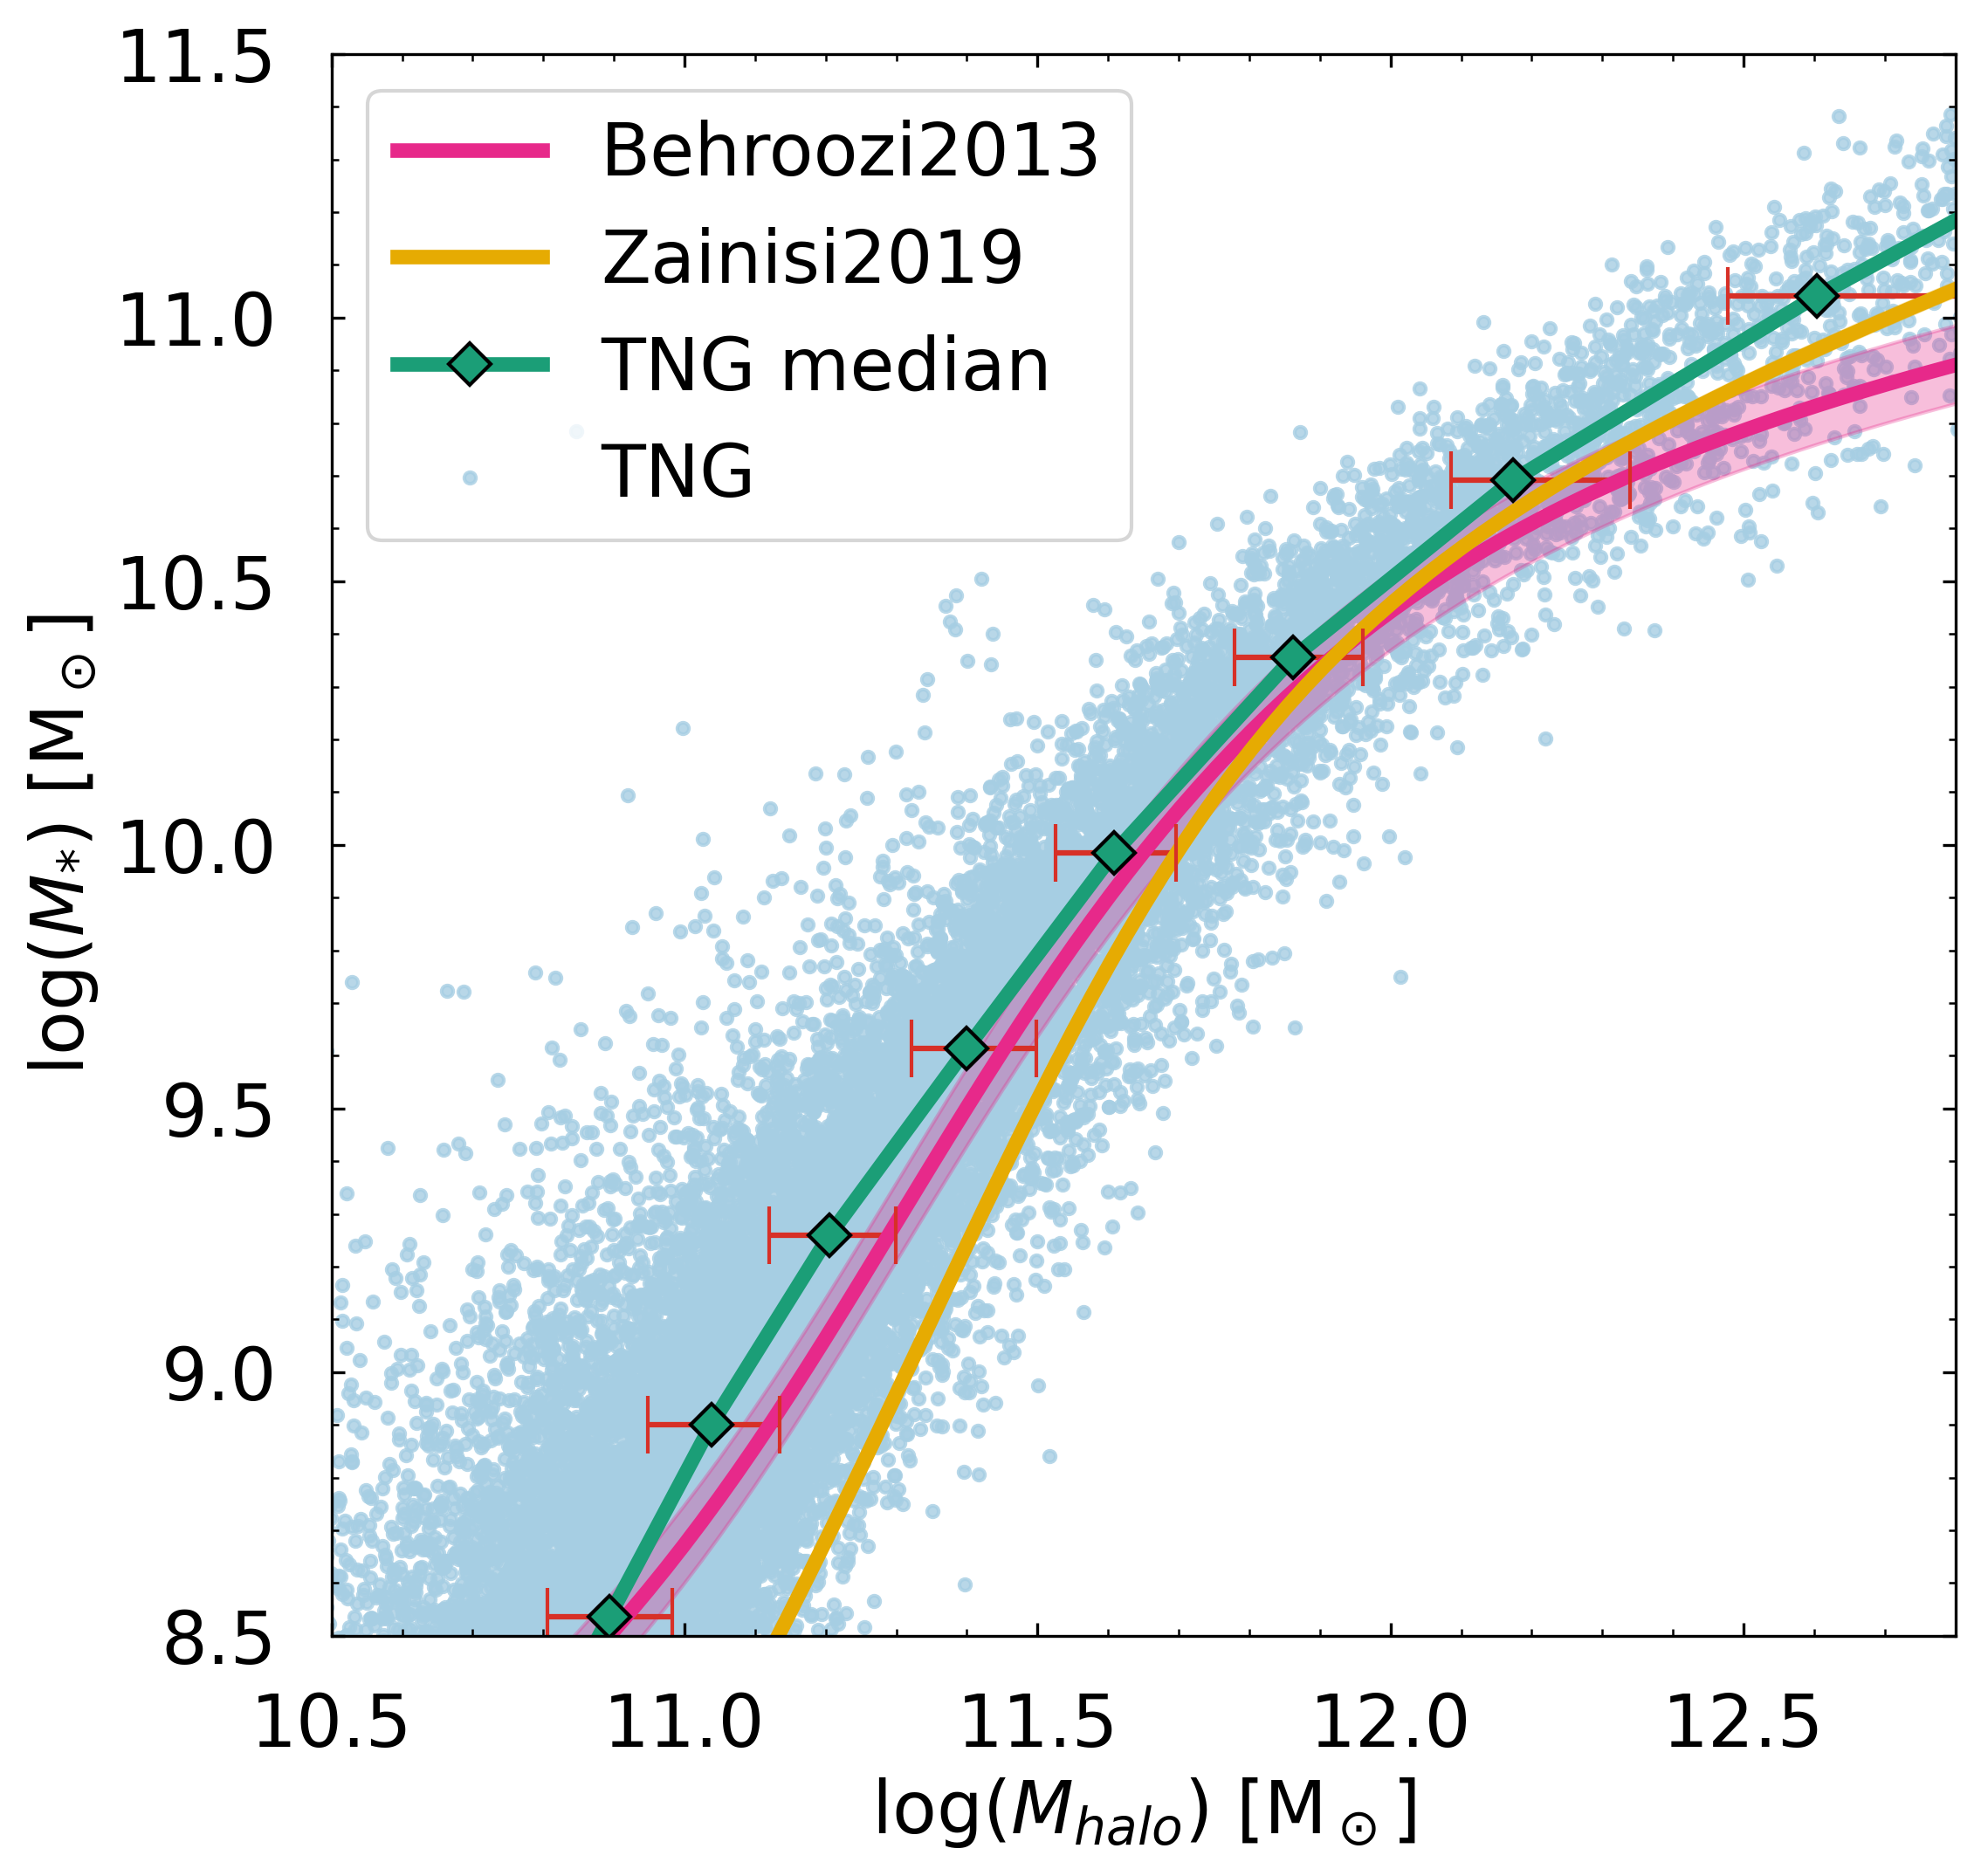
\includegraphics[width=0.9\paperwidth]{images/results_shmr.png}}
    \caption{The SHM relation of the TNG is shown (dots), along with median points (green) with error bars showing the 25-75 percentile. The best fit from abundance matching from \textcite{Behroozi2013} (dashed pink line) and \textcite{Zanisi2019} (yellow line)) are also shown.} 
    \label{shmr_res}
\end{figure}


\subsection{TFR}
The TFR for the late type galaxies in TNG is shown in Figure \ref{tfr_res} along with the best fit for the SAMI data found in \textcite{Bloom2017}. The linear fit to TNG data gives a slope of 4.13. This is steeper than that found in the SAMI data, which has a slope of 3.23. Rotational velocities for TNG are chosen as the maximum velocity in the velocity curve, while \textcite{Bloom2017}. use the velocity at $r = 2.2 r_e$. This could lead to the velocity measurements of the smaller galaxies being systematically lower compared to TNG. A better comparison would be to choose the same definition for the rotational velocity for both data sets. Also, it might be interesting to investigate the Baryonic Tuller-Fisher relation by adding the HI-mass and velocity measurements to the stellar measurements.

\begin{figure}
    \centering
    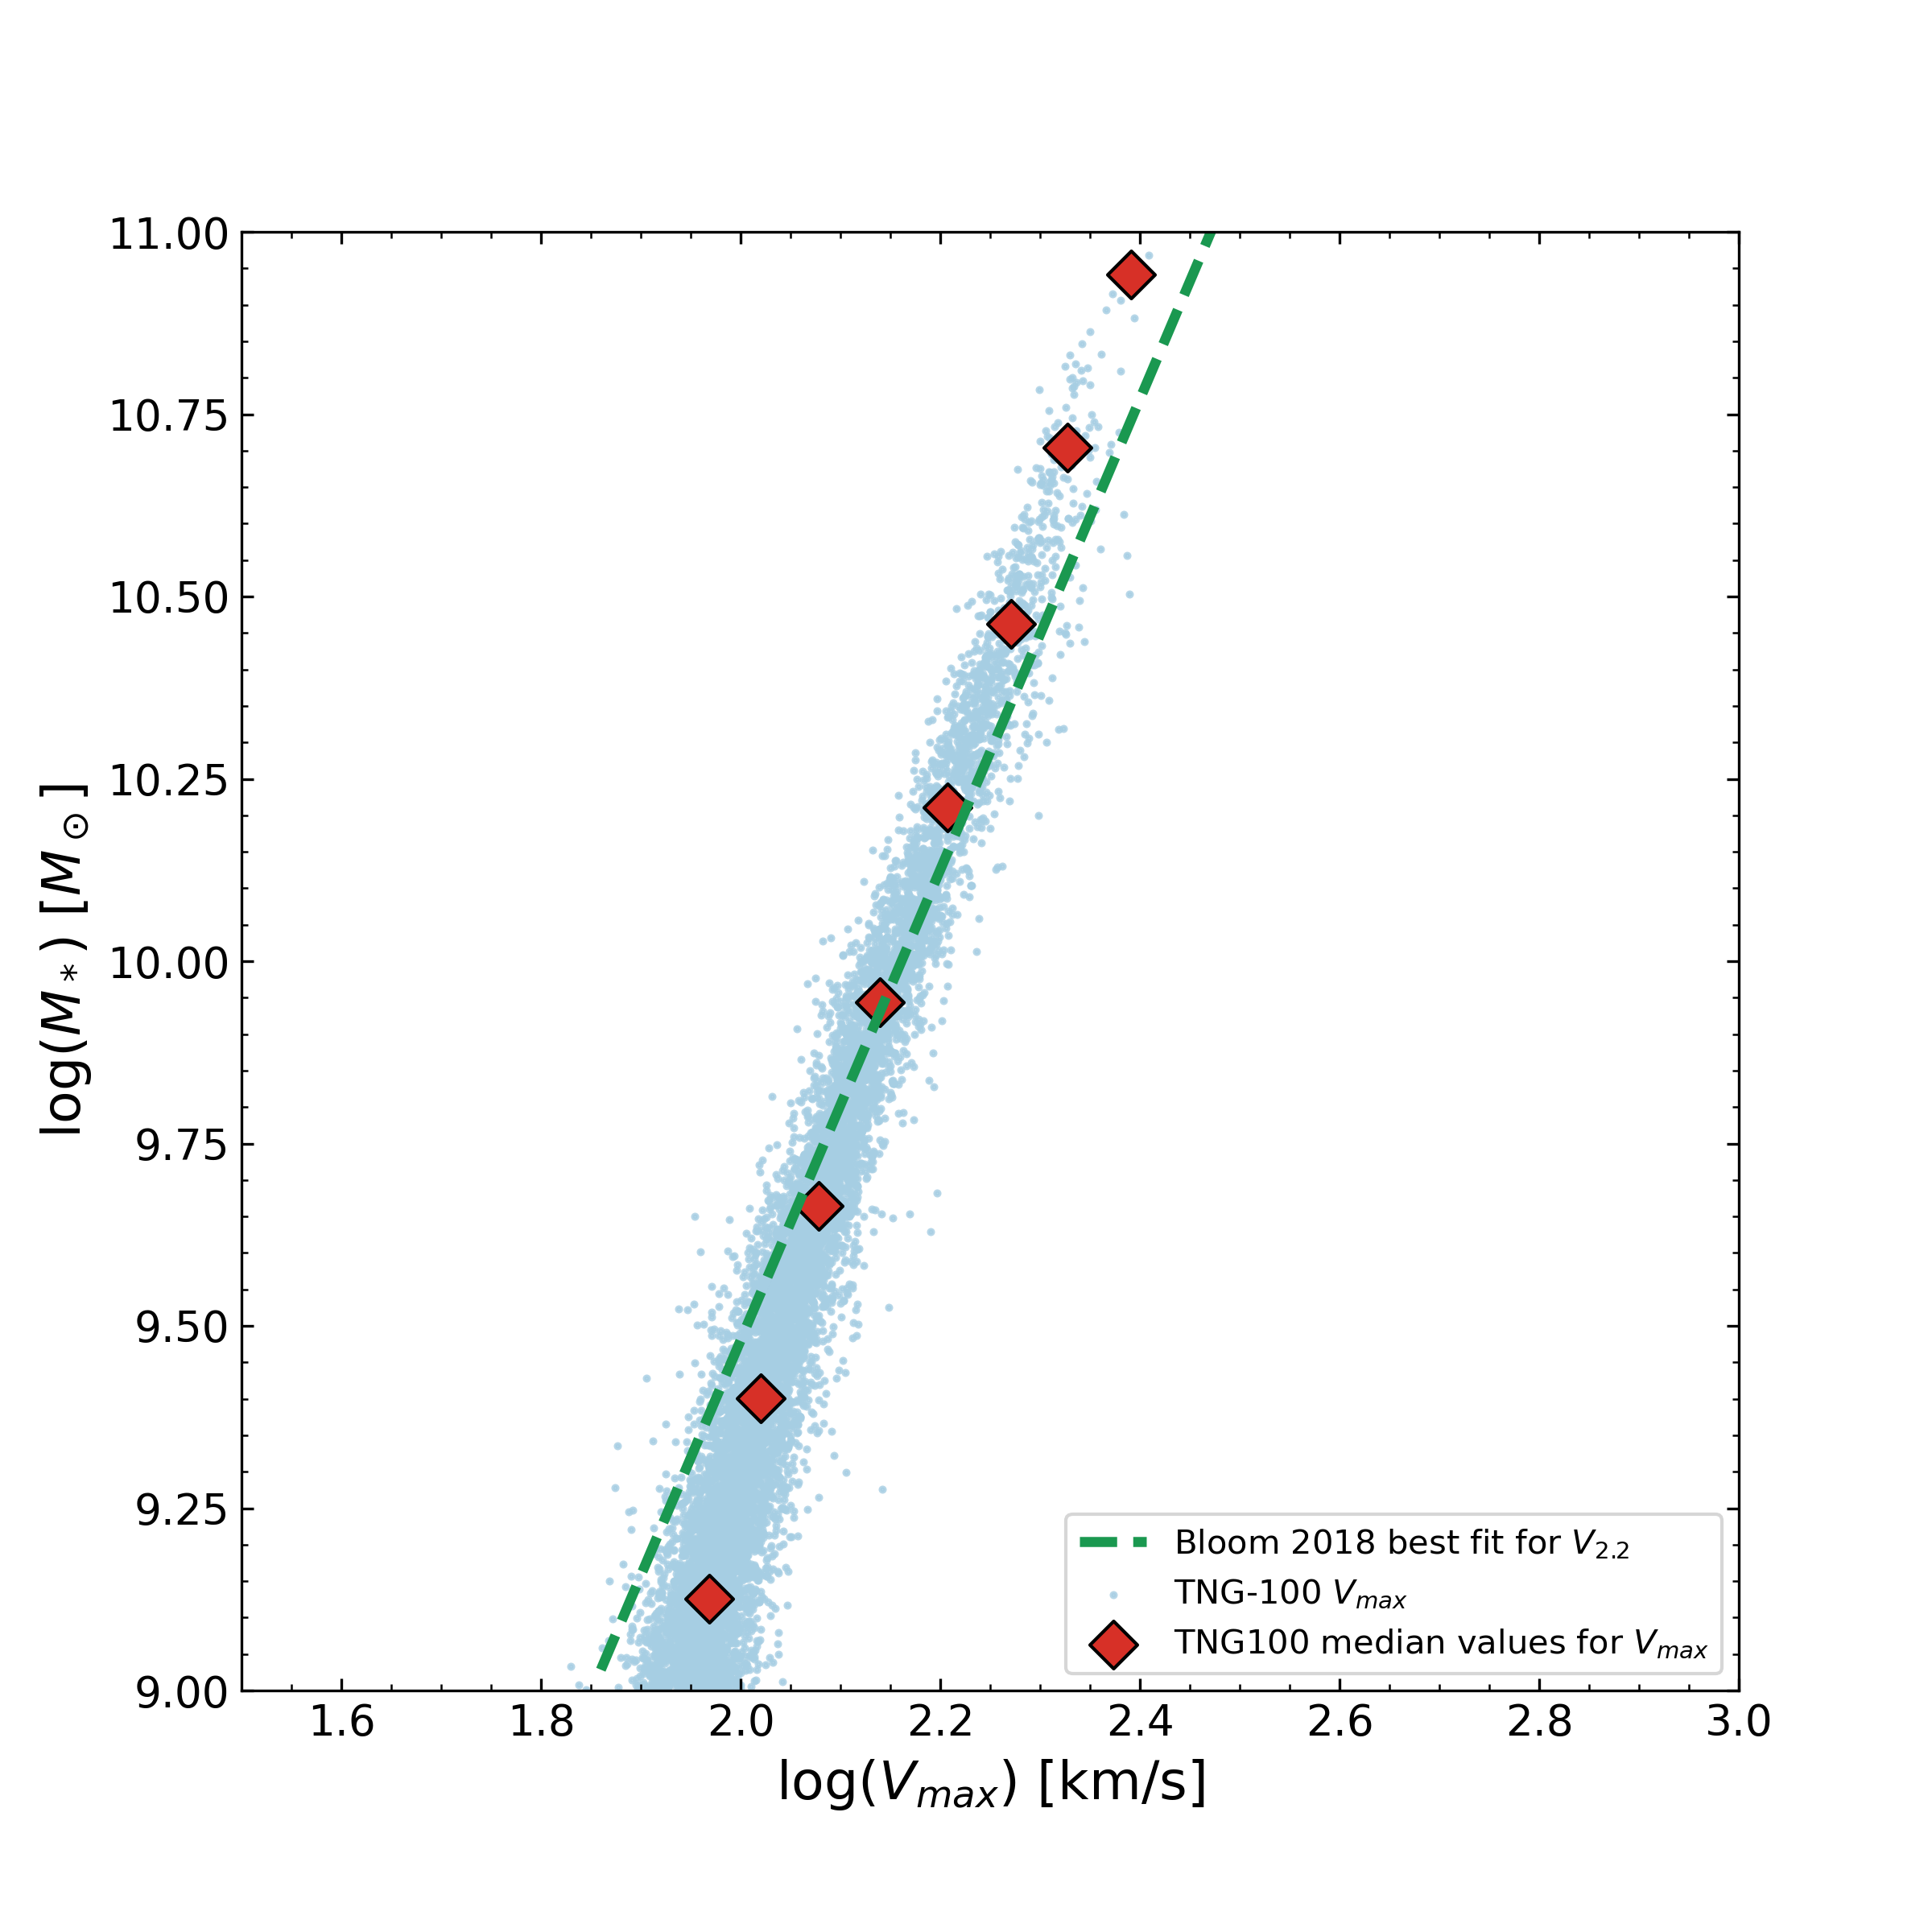
\includegraphics[width=0.9\textwidth]{images/results_tully_fisher.png}
    \caption{The TFR for TNG (blue dots). The median points are plotted with error bars, showing the 25-75 percentile. A linear fit is also provided (blue line). The best fit for the TFR using the SAMI data is also shown (dashed line).}
    \label{tfr_res}
\end{figure}

\subsection{FJ relation and the FP}

The velocity dispersion as function of stellar mass can be seen in Figure \ref{FJ_res}. The trend for the TNG data is a clear power law as expected from the FJ relation. Using linear regression the slope was found to be 3.14, with a y-intercept of 4.21. Compared to the observational data, the simulation data shows lower $\sigma$ values, by about 0.1-0.2 dex. This could be explained by the fact that the velocity dispersion in TNG galaxies is averaged across all particles identified by subfind and not only in the inner part of the galaxy. In general, gas has a lower $\sigma$ than stars and dark matter, so this could push the total $\sigma$ down. However, in early-type galaxies there is little gas so the impact would be expected to be small. The fact that $\sigma$ is found by averaging across the entire subhalo would include particles further out than for the SAMI data in which the velocity dispersion is averaged inside the effective radius ($\sigma_{e}$). Other studies have also found that simulations tend to get lower values for $\sigma$ \parencite{Sande2018}, so this might also just be a limitation of the simulations.

The other relations in the fundamental plane are shown in Figures \ref{FP_res1} and \ref{FP_res2}. 
/////////////
For galaxies with $M_*<10^9 M_{\odot}$, there are so few data points for SAMI that the comparison is not really meaningful. 

The $\sigma$-radius relation is also affected by the systematically lower $\sigma$ values for TNG. 

\begin{figure}
    \centering
    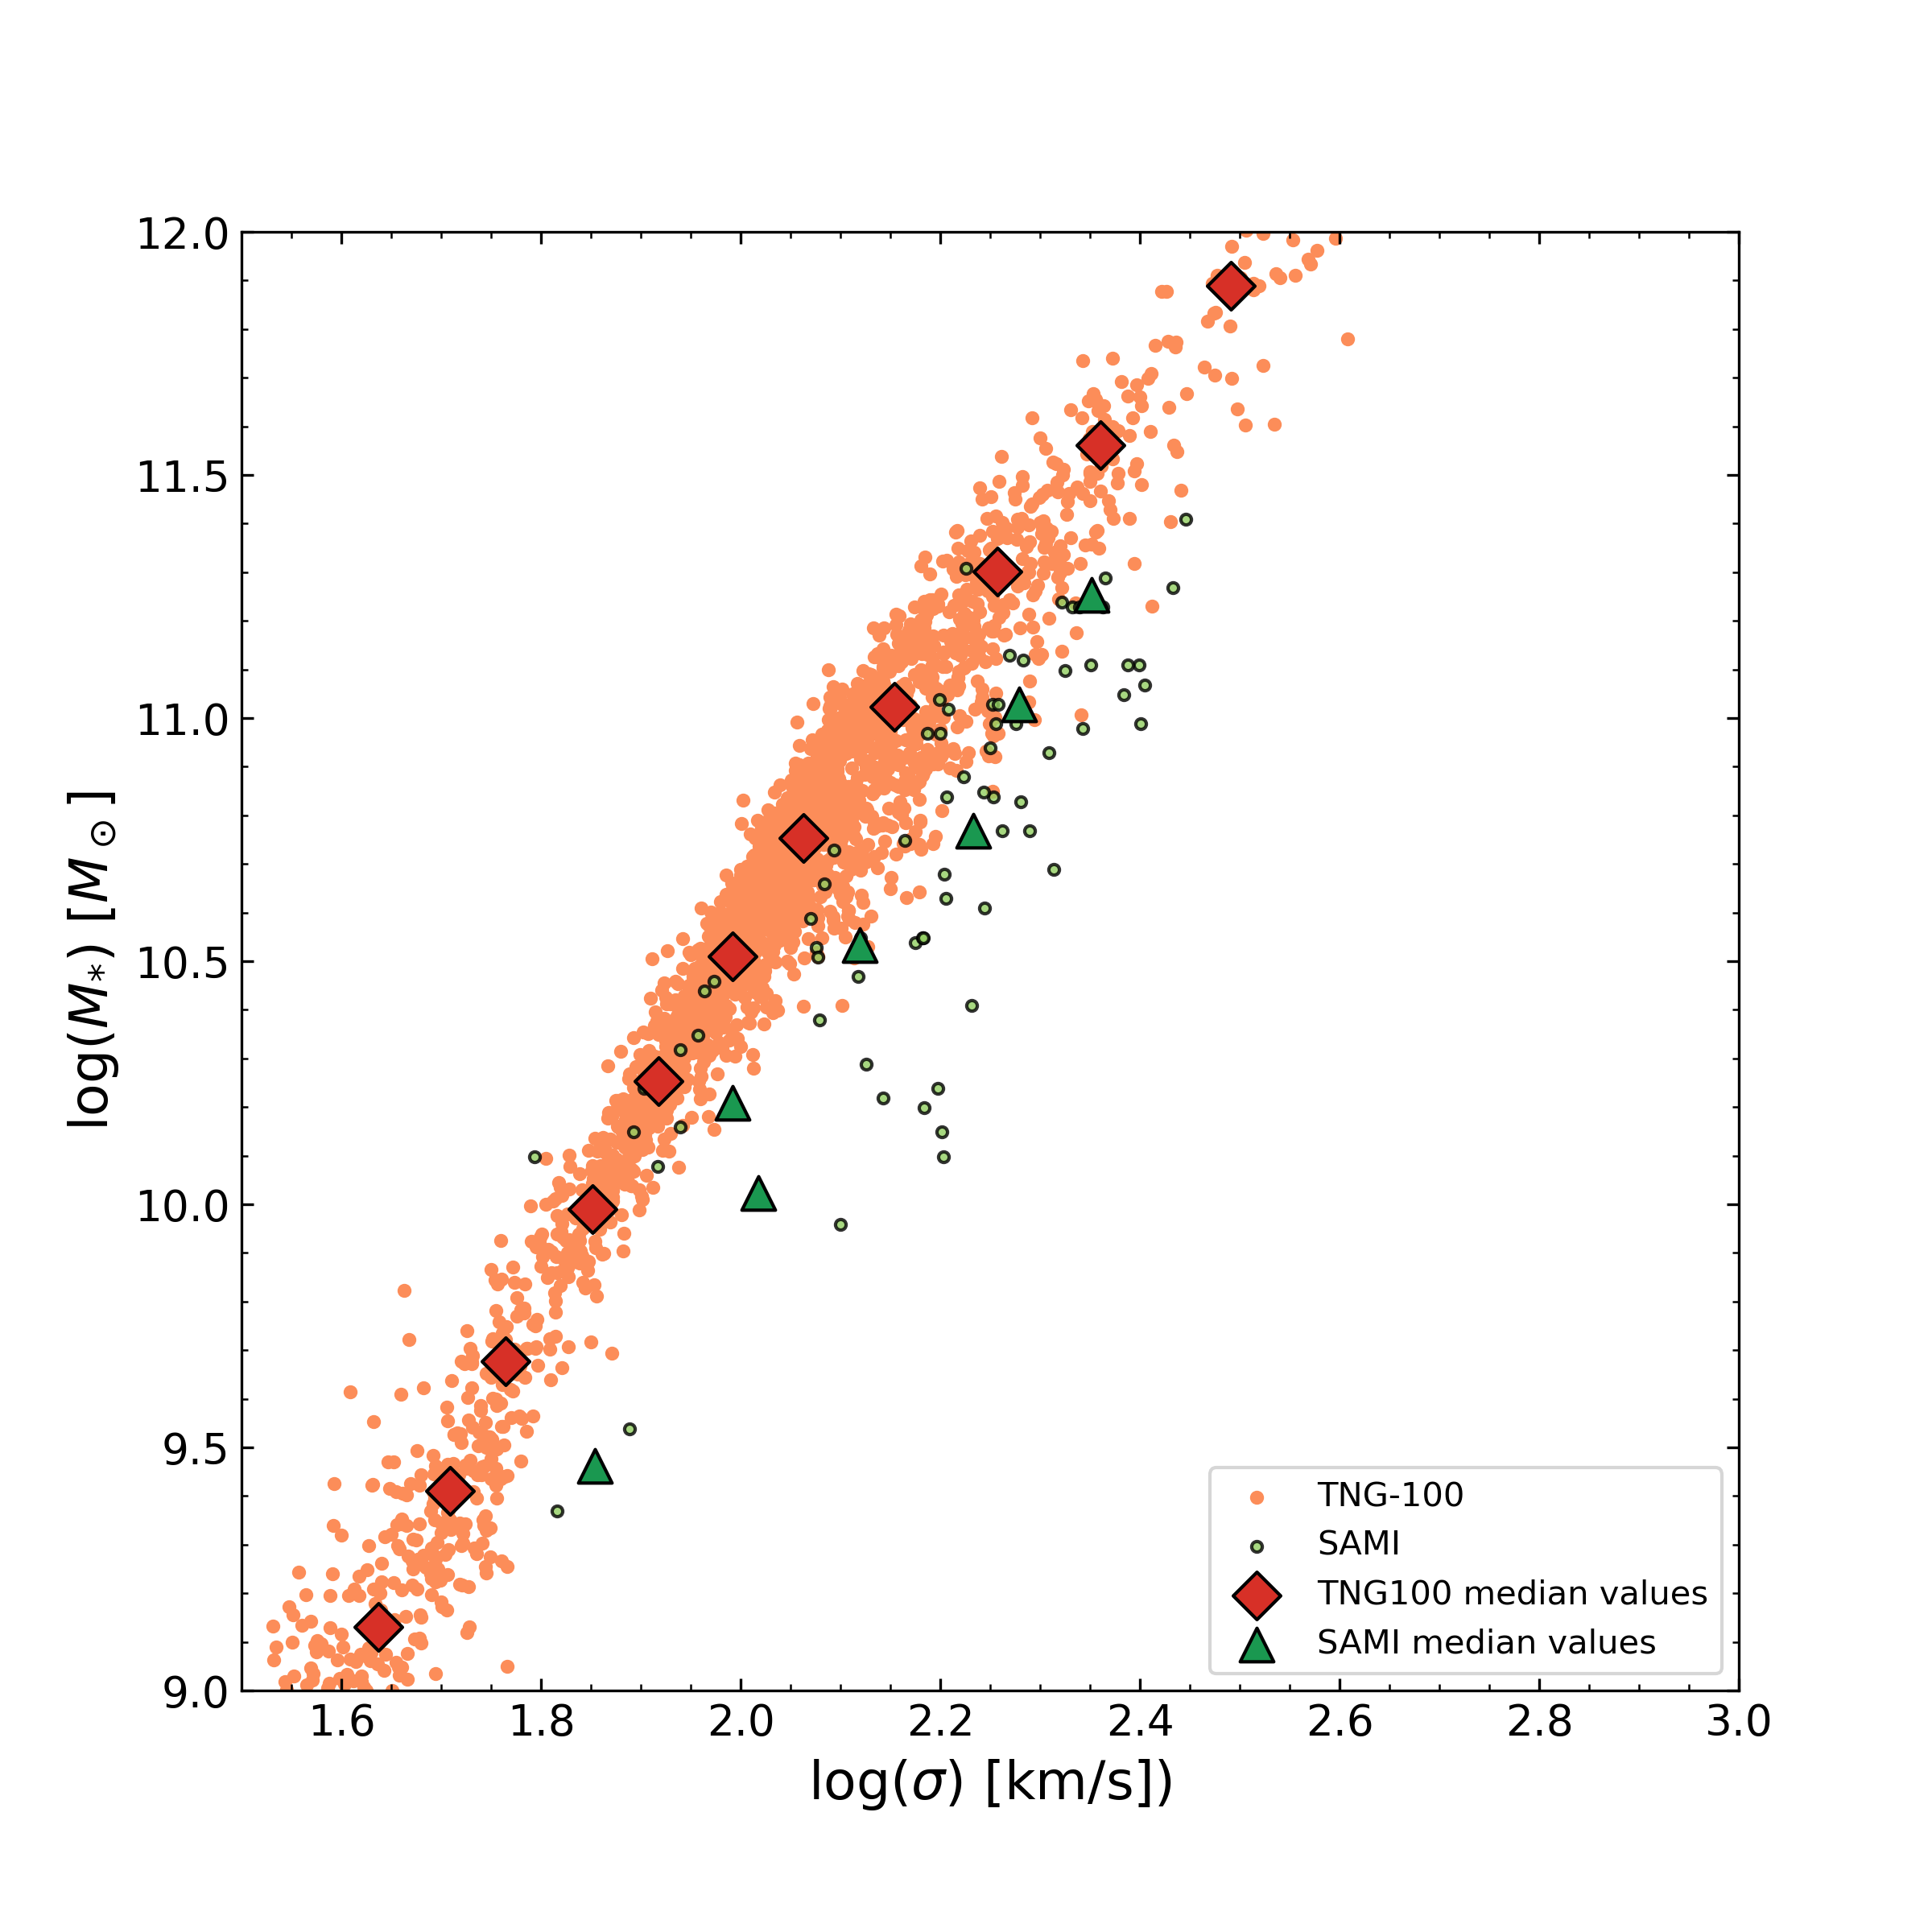
\includegraphics[width=\textwidth]{images/results_faber_jackson.png}
    \caption{The FJ relation in early type galaxies. The whole data set, as well as average values are shown for both TNG and SAMI.}
    \label{FJ_res}
\end{figure}

\begin{figure}
    \centering
    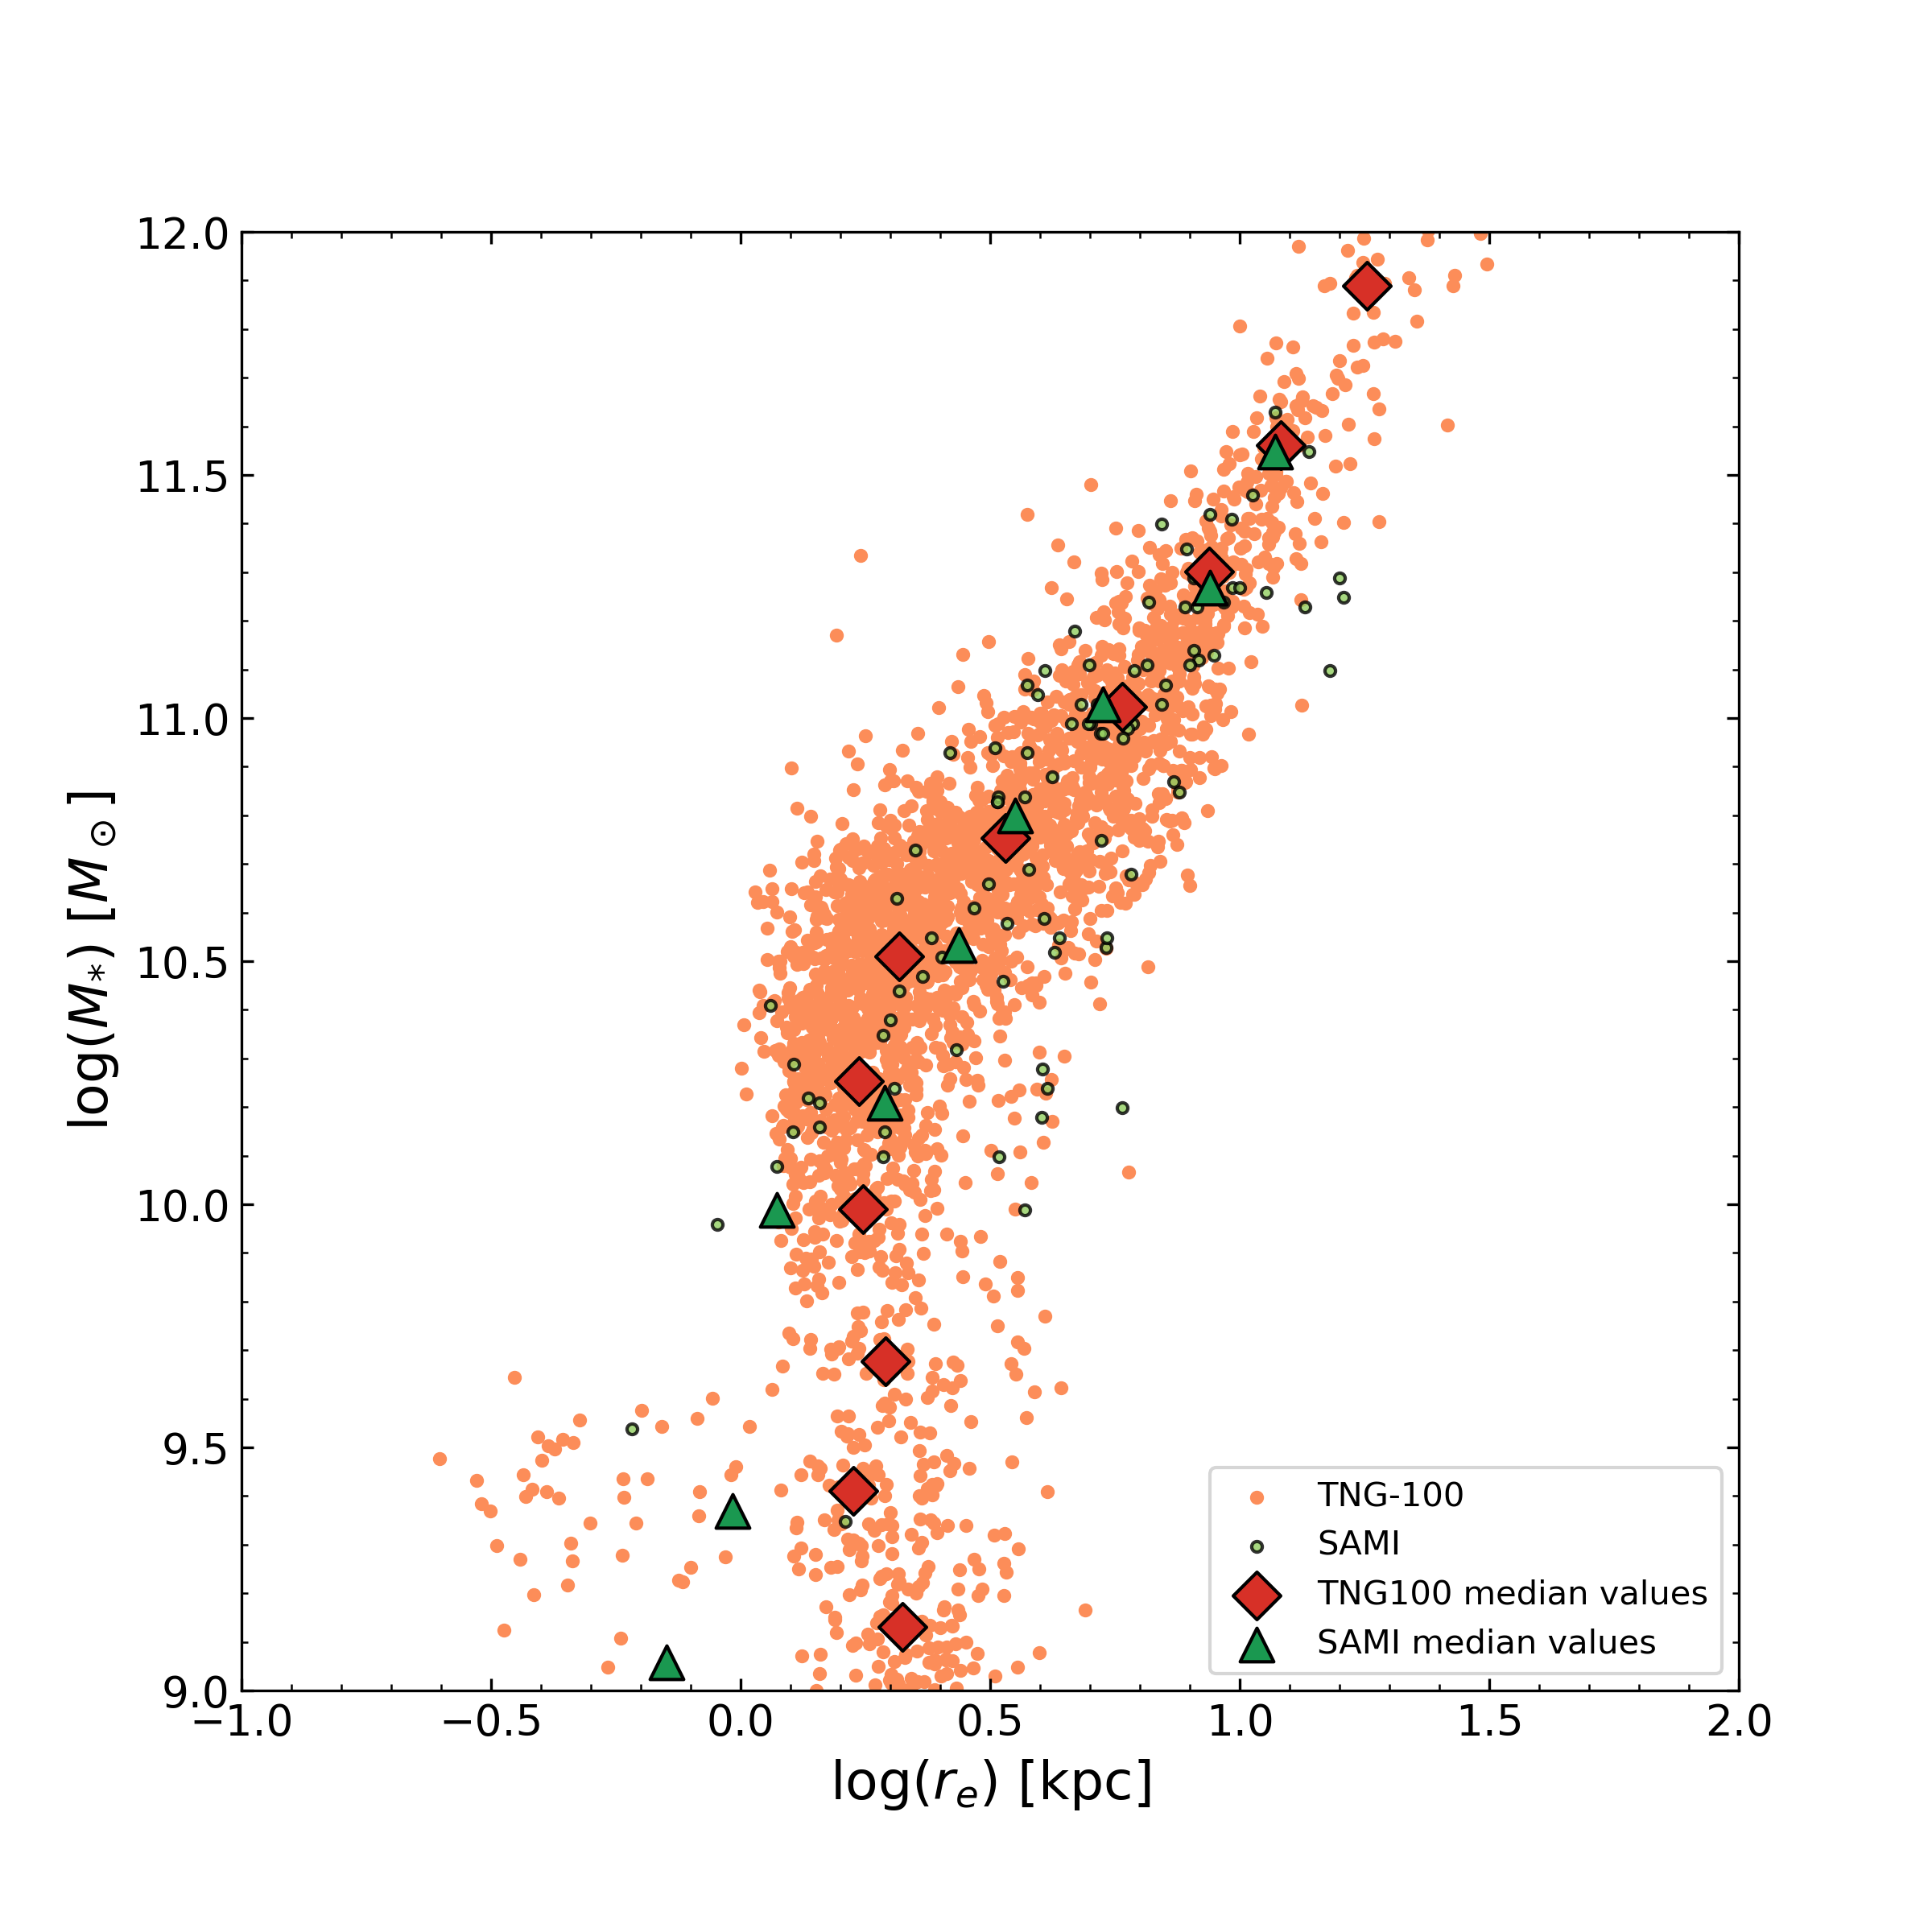
\includegraphics[width=\textwidth]{images/results_mass_radius_FP.png}
    \caption{Stellar mass as a function of effective radius.}
    \label{FP_res1}
\end{figure}

\begin{figure}
    \centering
    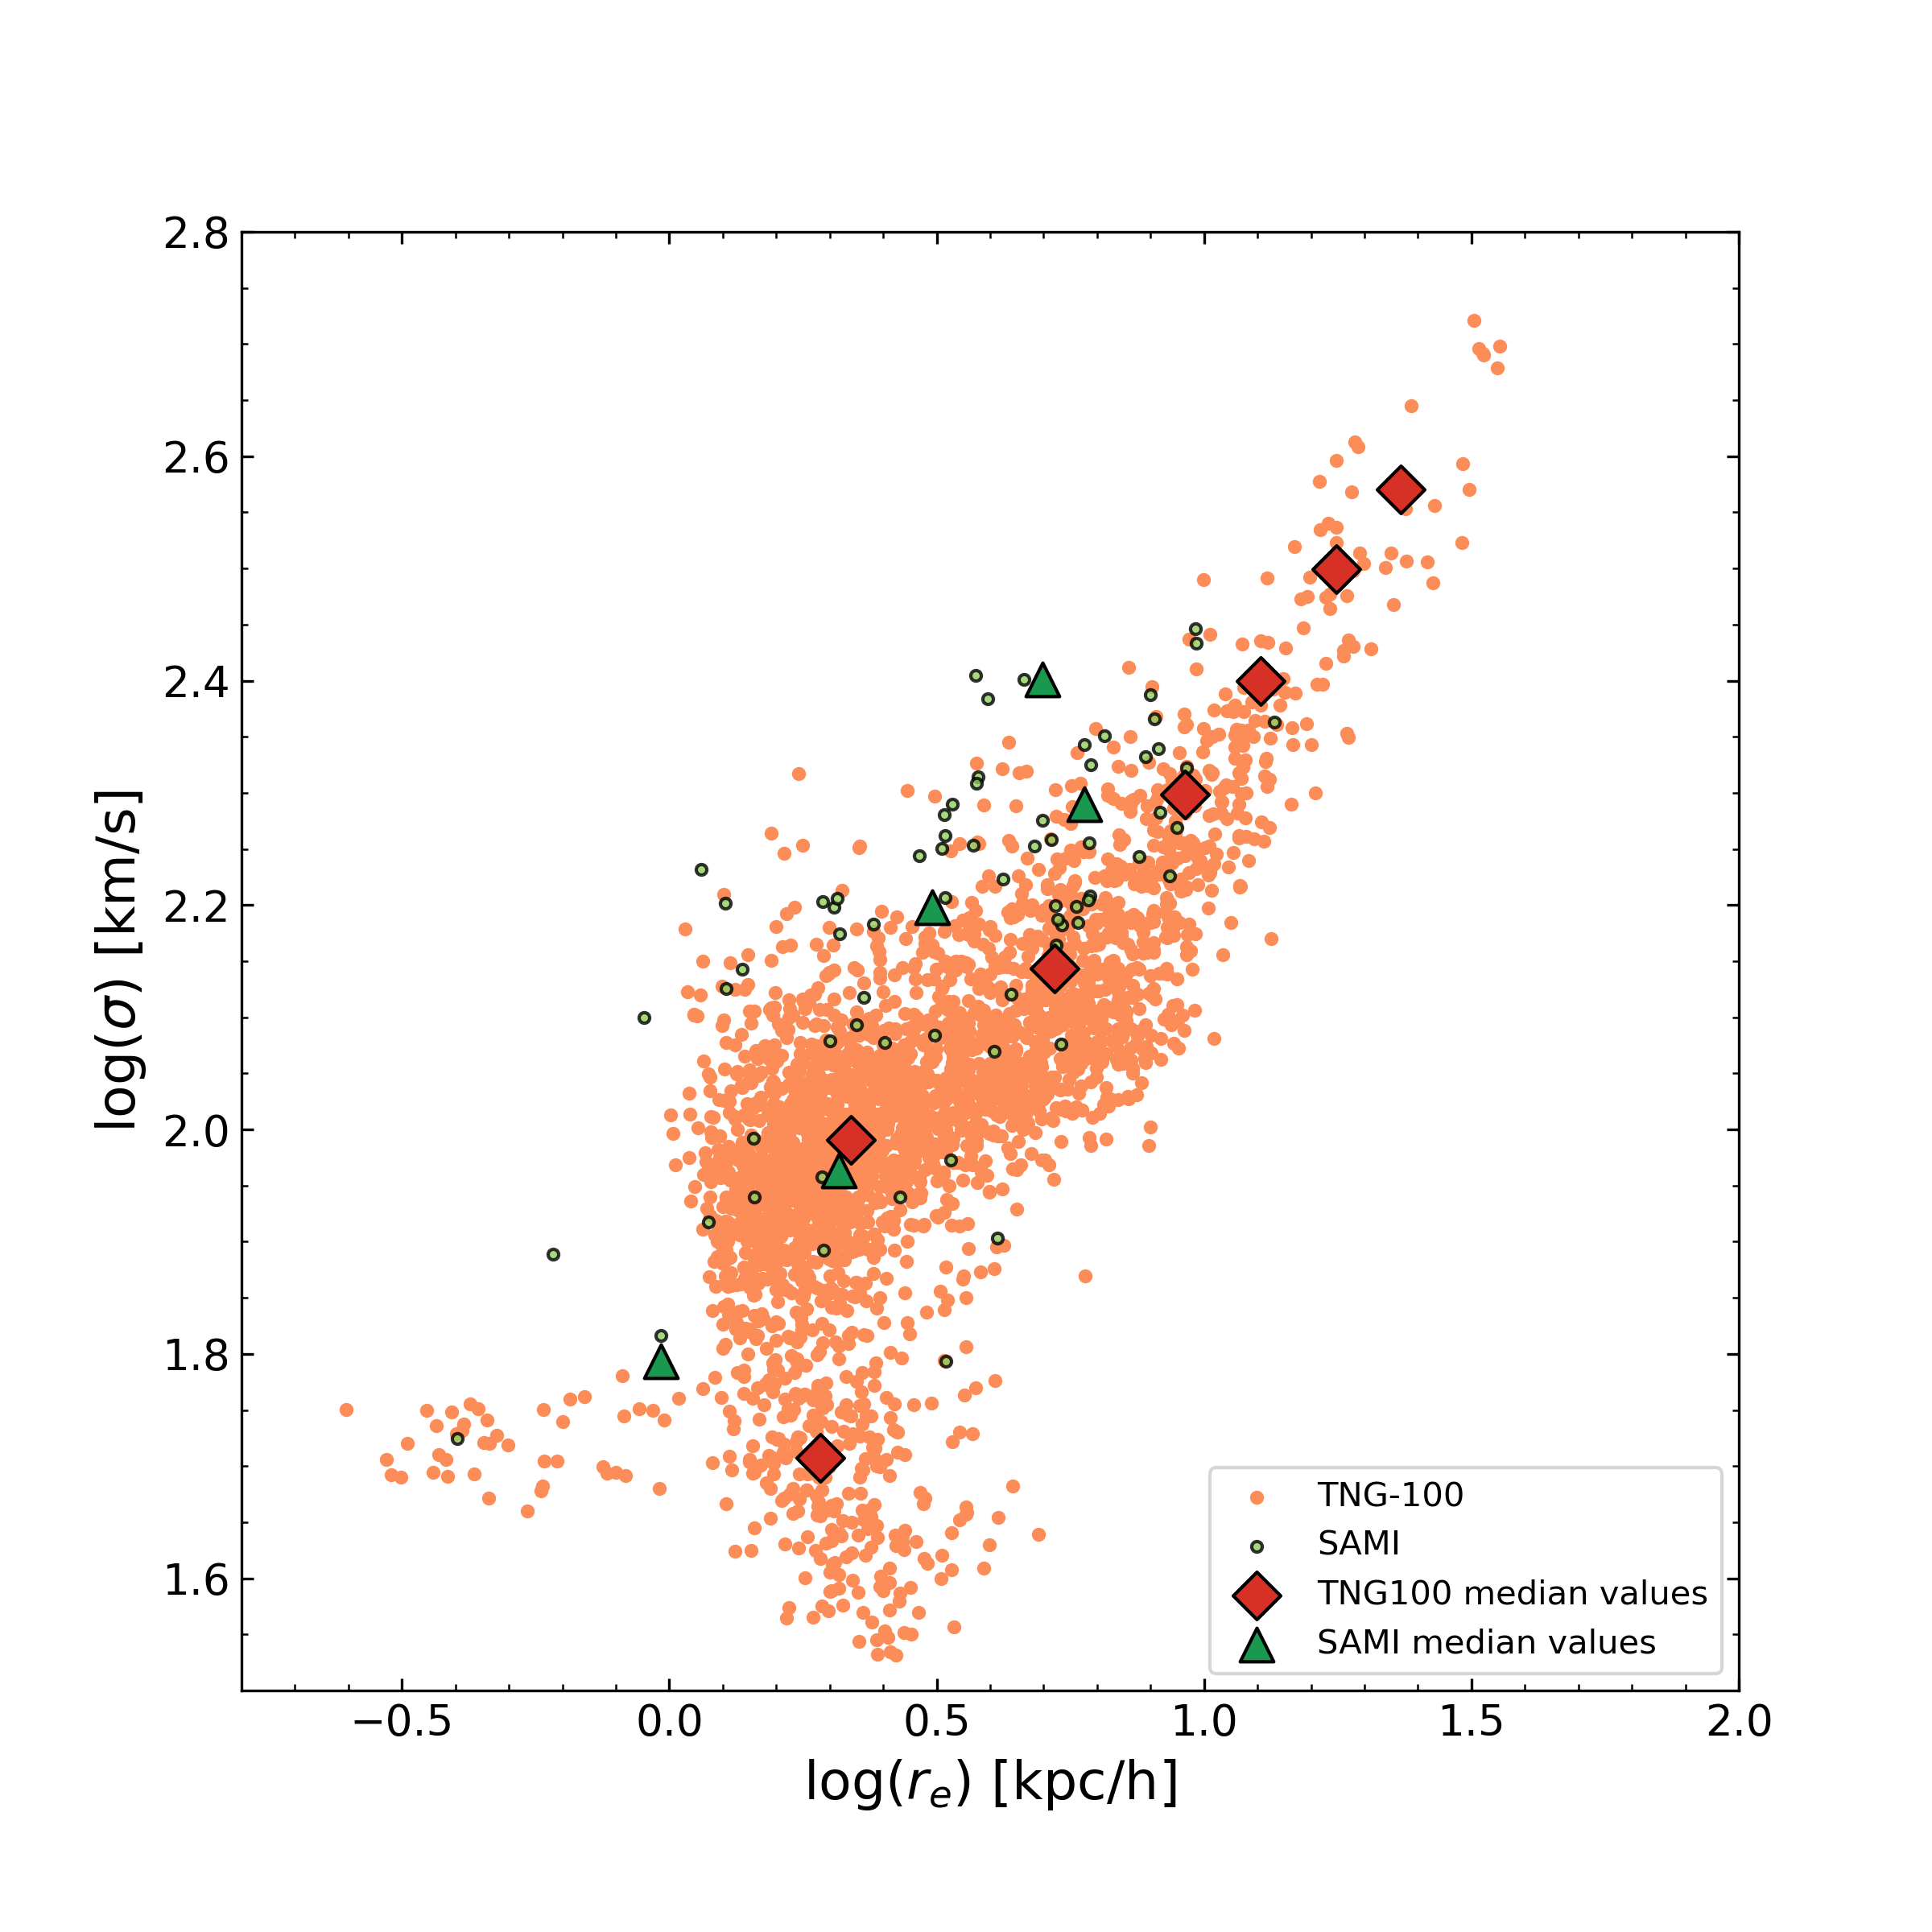
\includegraphics[width=\textwidth]{images/results_sigma_radius_FP.png}
    \caption{Velocity dispersion as a function of effective radius for early type galaxies.}
    \label{FP_res2}
\end{figure}

\subsection{Color bimodality}
The color-mass diagrams for different filters are shown in Figure \ref{color_magnitude_res}. There is a distinct seperation between early and late type galaxies, as expected. The distinction is clear in all bandfilters. 

In Figure \ref{pdf_color} the PDF for the TNG and SAMI (g-i) color are shown. The peaks coincide well for the two data sets, although the distribution in galaxies is different. This is likely because TNG has a larger amount of smaller, late-type blue galaxies, which are much more difficult to observe than larger and generally redder galaxies. A mass weighted PDF might give a more fair comparison.

\begin{figure}
    \centering
    \makebox[\textwidth][c]{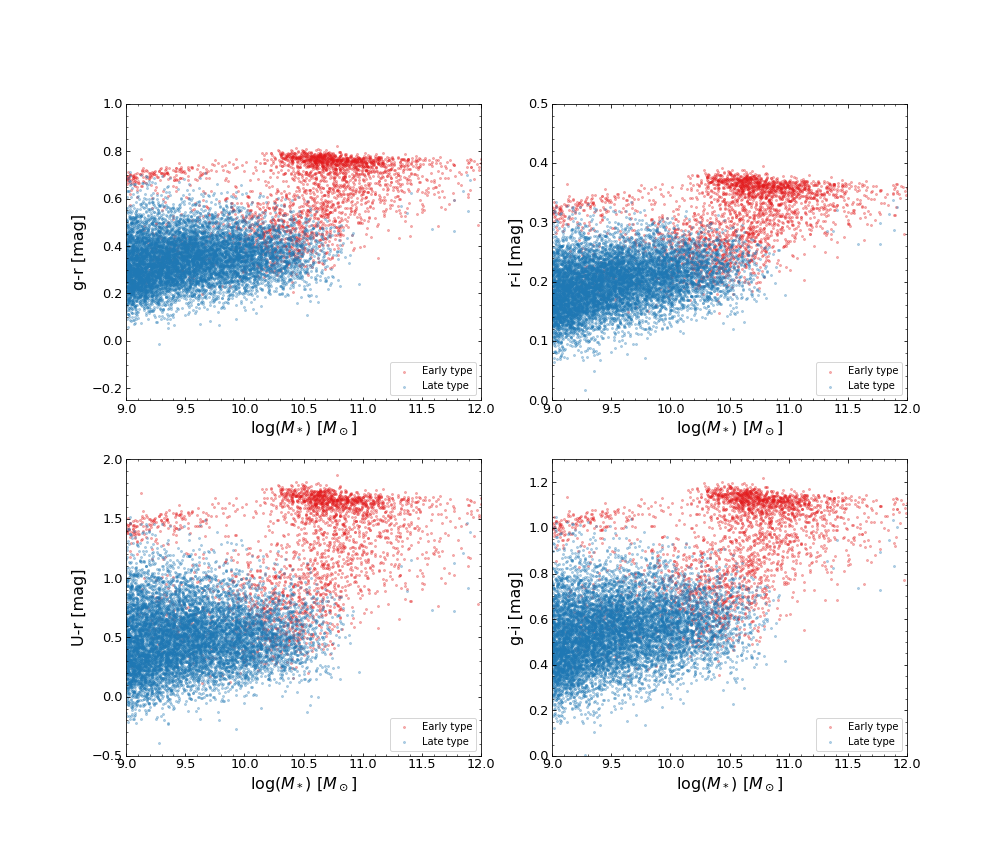
\includegraphics[width=0.9\paperwidth]{images/results_color_magnitude.png}}
    \caption{}
    \label{color_magnitude_res}
\end{figure}


\begin{figure}
    \centering
    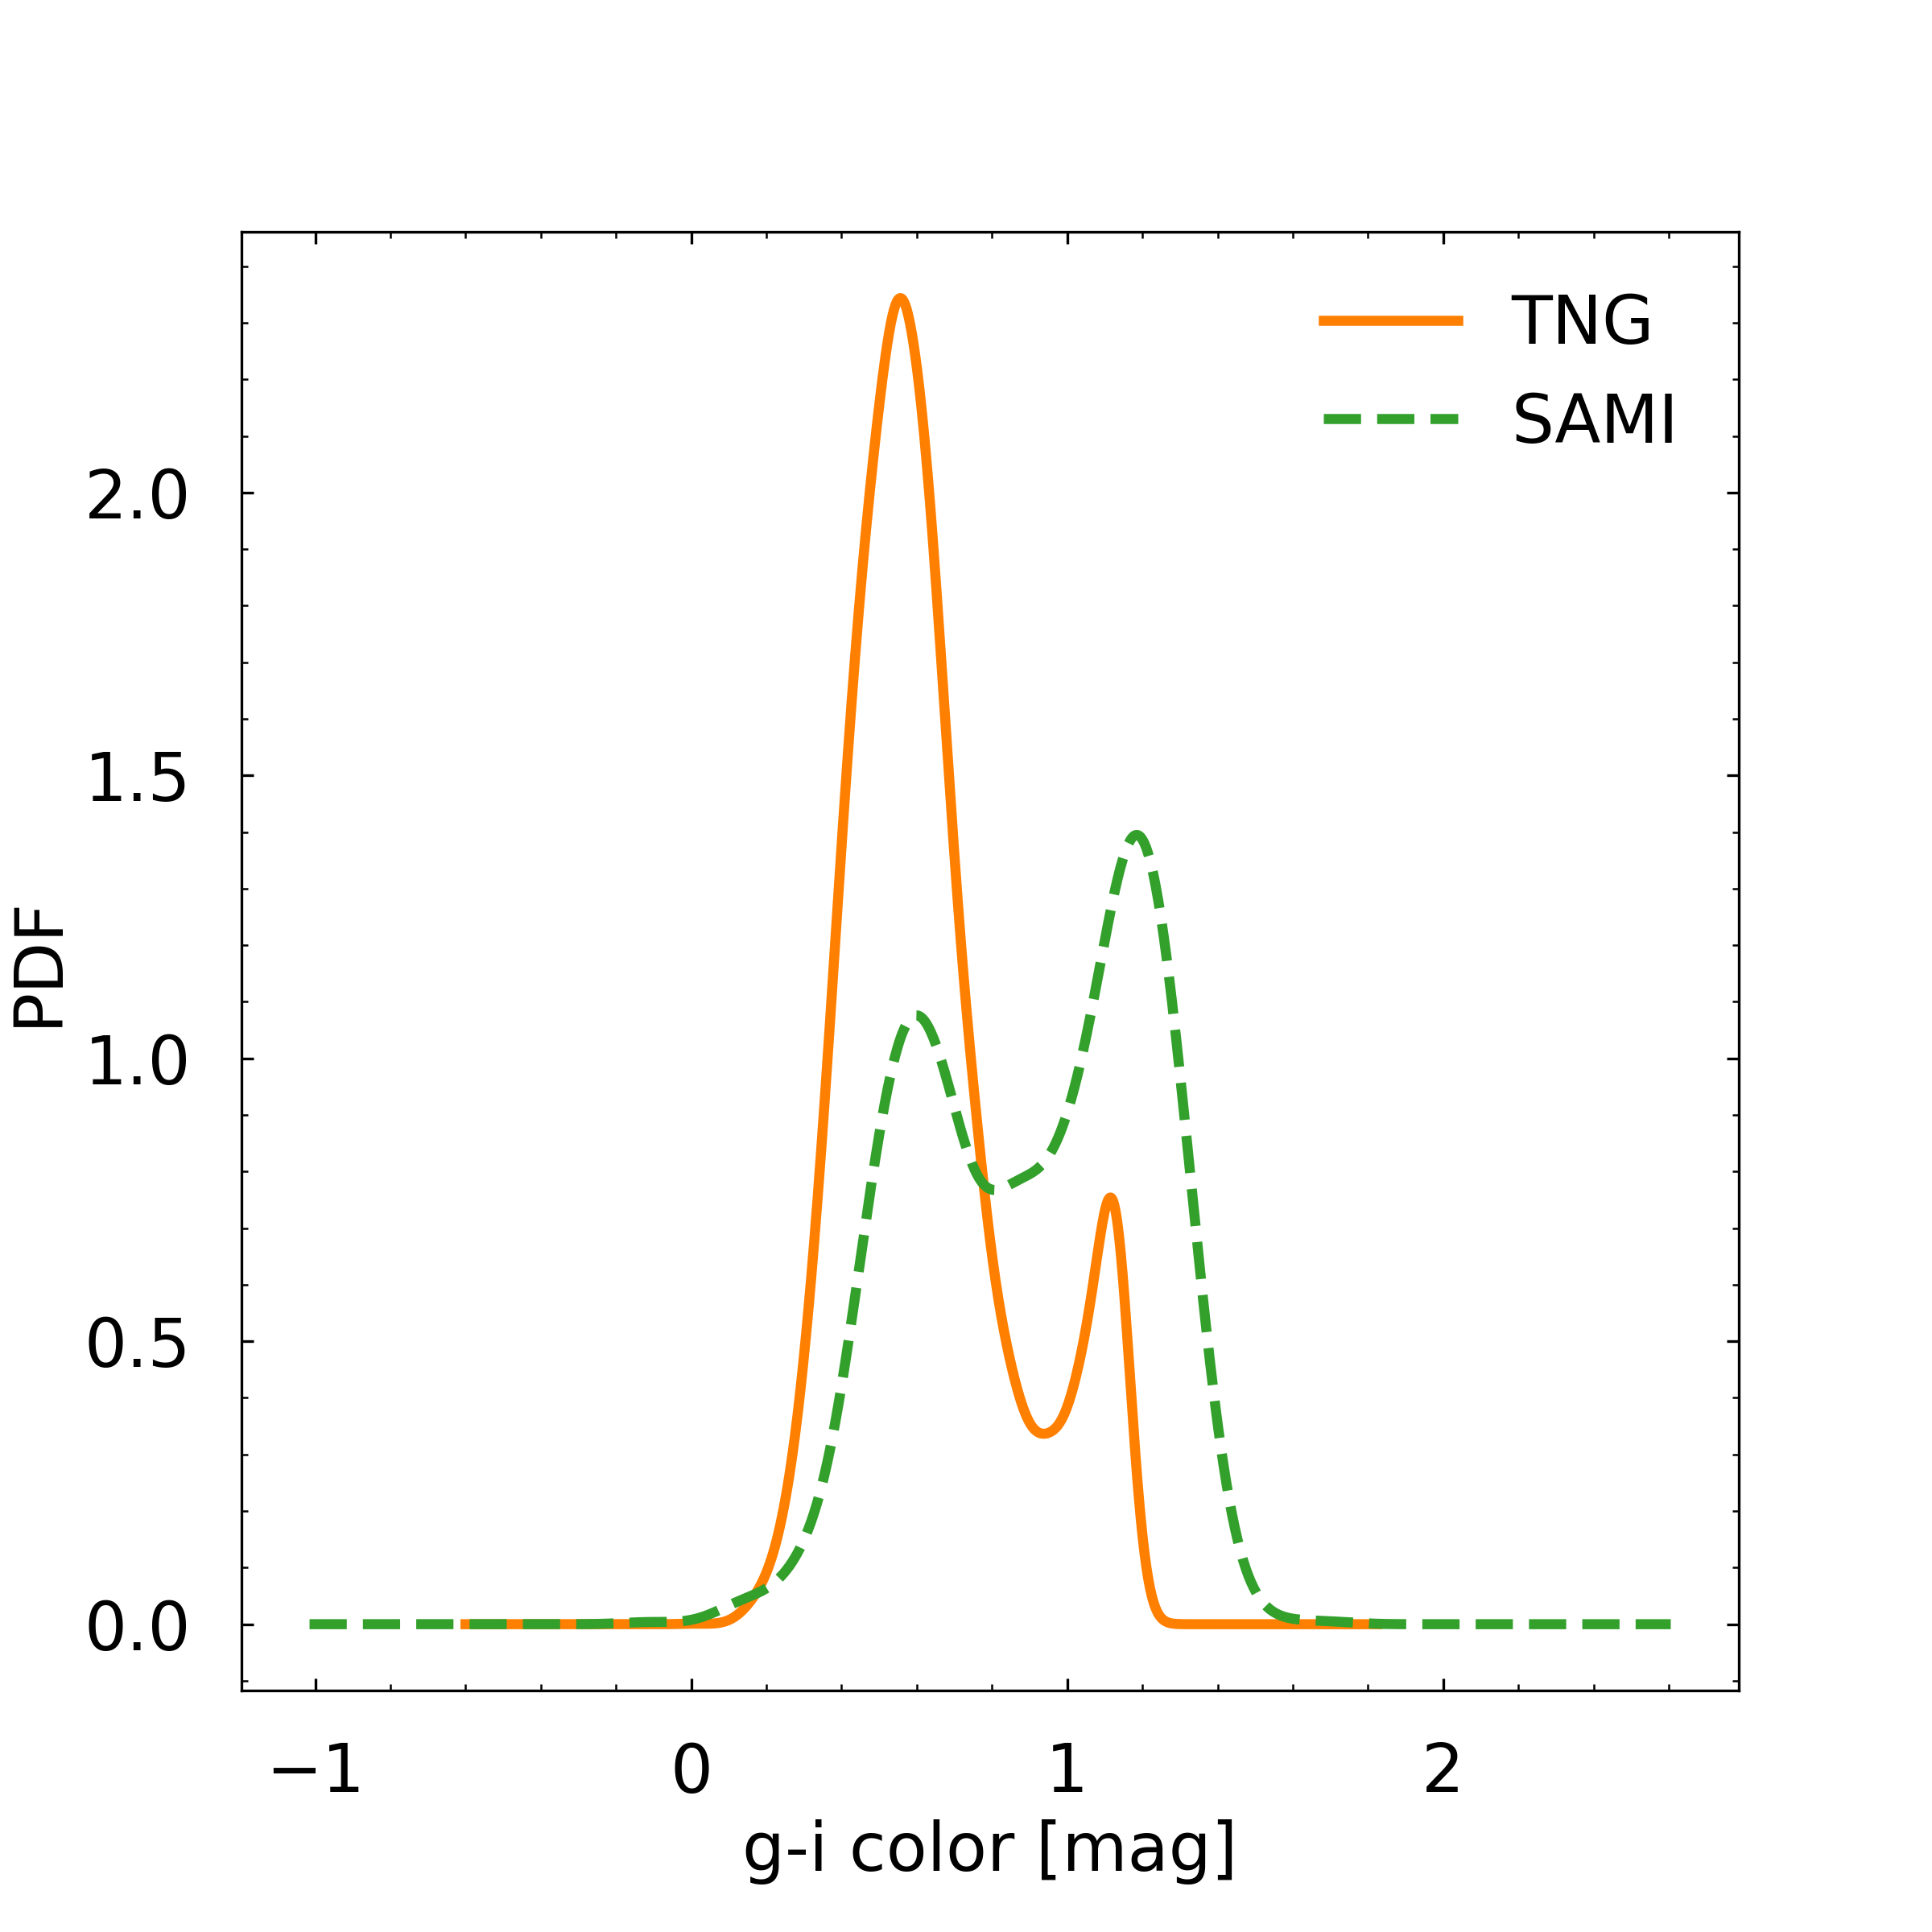
\includegraphics[width=0.9\textwidth]{images/results_pdf_g_i_band.png}
    \caption{}
    \label{pdf_color}
\end{figure}

